%\section{Manipulating the Interval}

%Changing this to just be the ice-tea activity
\note{Timing: \unit[\about35]{min}}{}
\section{Defining Appropriate Intervals for Analysis}
\label{act1.2.3}

\begin{overview}

\textbf{Overview:} Remember that we \hyperref[act1.2.2D]{talked about} how asking different questions makes us choose different intervals of interest for our investigations using the \EnergyInteractionModel? Here, we'll explore this issue a bit further.

\end{overview}

% We already did this activity and \FNT{} in D/L 4. Commenting this out here.
%\subsection{}
%
%\begin{FNTenv}
%	\input{U1/FNT1.2.1-4}
%\end{FNTenv}

%\note{Timing: \unit[\about10]{min}}{
	
%}

%\begin{enumerate}
%	\item Why is it {\em not} possible to apply the \textbf{\EnergyInteractionModel{}} in a straightforward way to the interval of interest? (The interval that ends when all of the \unit[252]{kJ} has been added to the water.) In other words, why can't the overall interval be diagrammed using {\em only} the given information prior to doing any further analysis?   Draw a \TempGraph{} to help you make sense of this and to use to explain it. In particular, be sure to make explicit which part of the graph in the diagram refers to which ``energy bubble'' on the \EnergyDiagram{}. \textbf{[To save time, it is ok for explanations on the board to be more fragmentary and shorthand than explanations on exams, because anything that is unclear can be easily clarified in the Whole Class Discussion.]}
	
%	\item Explain how to use the \EnergyInteractionModel{} to analyze {\em shorter intervals} in order to determine the final state (phase and temperature) of the \ce{H2O}. Use a \TempGraph{} in your analysis and to use in your explanation.
%\end{enumerate}

%\WCD 

%\subsection{Two objects coming to thermal equilibrium}
\todo[inline]{Notes on Ice-Tea activity

	Needs to be restructured as chart addition doesn't fit well. Perhaps do original ice tea activity and THEN do chart if time?}

\noindent\textbf{Consider the following phenomenon:} A \textbf{big} chunk of ice (water) at an initial temperature of  \unit[-65]{\textdegree C} is placed inside a well-insulated container with some tea at an initial temperature of \unit[20]{\textdegree C}, and the two are allowed to come to thermal equilibrium. (The tea can be treated as water with respect to thermal properties.)



\begin{enumerate}
	\item There are several possible final states of this process. We will be using and reusing the same \ThreePhaseModel{} to determine possible final states. Draw two \TempGraphs{}, one for tea and one for \ce{H2O}.
	\begin{enumerate}
		\item Why can't either substance reach thermal equilibrium in the gaseous phase nor the mixed (liquid/gas) phase nor the gaseous phase?
		\label{act123a}
		\item Using the \hyperref[act123-grid]{grid below}, your instructor will assign your group one of the potentially possible final states. Trace your \TempGraph{} to show how your assigned ending phase is or is not possible.
		\label{act123-gridprob}
		\note{Create energy interaction diagramsfor \ref{act123a}}{
State 1: A LOT of ice would make this state possible b/c the tea would be cooled to a solid. A LOT of tea would make this state unlikely to happen b/c the tea�s final state is a solid in this instance and a little ice would not be cold enough to make the tea a solid
\\[0.25in]
State 2: A LOT of ice would make this state possible b/c the tea would be cooled enough to go through a phase change. However, a LOT of tea would make this state unlikely for the reason state above.
\\[0.25in]
State 3: A LOT of ice or a LOT of tea would make this state unlikely b/c it takes an exact amount of ice and tea to ensure the ice and tea lose transfer the same amount of thermal energy. 
\\[0.25in]
State 6 an 9: A LOT of ice would make this state unlikely b/c now the opposite is happening, we need the ice to go through a phase change and having a lot of ice would require a LOT of energy to do so. A LOT of tea would make this state likely b/c you would have enough tea for the little bit of ice to go through a phase change.
		}
	\end{enumerate}

\newcommand{\gridsize}{3cm}
\begin{table}[h]
	\caption{Grid for \ref{act123-gridprob}}
	\label{act123-grid}
	\begin{tabular}{cr>{\centering}b{\gridsize}>{\centering}b{\gridsize}b{\gridsize}<{\centering}}
							&						& \multicolumn{3}{c}{\textbf{Tea}} \\
							&						& Solid 						& Mixed Phase\newline\scriptsize(Solid/Liquid) & Liquid \\\cline{3-5}
							&						& \multicolumn{1}{|l|}{i.} 			& \multicolumn{1}{|l|}{ii.}	& \multicolumn{1}{|l|}{iii.} \\
							& 						& \multicolumn{1}{|c|}{} 			& \multicolumn{1}{|c|}{}	& \multicolumn{1}{|c|}{} \\
							& Solid					& \multicolumn{1}{|c|}{} 			& \multicolumn{1}{|c|}{}	& \multicolumn{1}{|c|}{} \\
							& 						& \multicolumn{1}{|c|}{} 			& \multicolumn{1}{|c|}{}	& \multicolumn{1}{|c|}{} \\
							& 						& \multicolumn{1}{|c|}{} 			& \multicolumn{1}{|c|}{} 	& \multicolumn{1}{|c|}{} \\\cline{3-5}
							&  						& \multicolumn{1}{|l|}{iv.} 			& \multicolumn{1}{|l|}{v.}	& \multicolumn{1}{|l|}{vi.} \\
\multirow{3}{*}{\rotatebox[origin=l]{90}{\textbf{Ice}}}	& 	 		& \multicolumn{1}{|c|}{}			& \multicolumn{1}{|c|}{} 	& \multicolumn{1}{|c|}{} \\
							& Mixed Phase				& \multicolumn{1}{|c|}{} 			& \multicolumn{1}{|c|}{}	& \multicolumn{1}{|c|}{} \\
							& \scriptsize(Solid/Liquid)		& \multicolumn{1}{|c|}{} 			& \multicolumn{1}{|c|}{}	& \multicolumn{1}{|c|}{} \\
							&  						& \multicolumn{1}{|c|}{} 			& \multicolumn{1}{|c|}{}	& \multicolumn{1}{|c|}{} \\\cline{3-5}
							&  						& \multicolumn{1}{|l|}{vii.} 			& \multicolumn{1}{|l|}{viii.}	& \multicolumn{1}{|l|}{ix.} \\
							& 	 					& \multicolumn{1}{|c|}{} 			& \multicolumn{1}{|c|}{}	& \multicolumn{1}{|c|}{} \\
							& Liquid					& \multicolumn{1}{|c|}{} 			& \multicolumn{1}{|c|}{}	& \multicolumn{1}{|c|}{} \\
							&  						& \multicolumn{1}{|c|}{} 			& \multicolumn{1}{|c|}{}	& \multicolumn{1}{|c|}{} \\
							&  						& \multicolumn{1}{|c|}{} 			& \multicolumn{1}{|c|}{}	& \multicolumn{1}{|c|}{} \\\cline{3-5}
	\end{tabular} 
\end{table}
\note{Grid solution for \ref{act123-gridprob}}{
\begin{center}
\begin{tabular}{c|c|c|c|}
 ICE \textbackslash Tea& Solid & Mixed & Liquid \\
 \hline
 Solid & i. Many possible temperatures & Many possible phases & Exactly one temp \& phase \\
 \hline
 Mixed & iv. No (can't cross) & v. No (see below) & vi. Many possible phases  \\
 \hline
 Liquid & vii. No (can't cross) & vii. No (can't cross) & viii. Many possible temperatures  \\
 \hline
\end{tabular}
\end{center}
\label{default}
By ``Can�t cross'' I mean that the final states of the ice and tea actually cross one another on the three phase diagram. This isn�t possible because the energy transfer will stop once the ice and the tea reach the same temperature.
\\[0.25in]
Final State v. Similarly, this state isn�t possible because if one substance is in the mixed S/L phase, then the other substance will stop at the corner once it reaches the melting point because the ice and the tea are at thermal equilibrium.

%	\begin{center}
%		\label{teaandicechart}
%		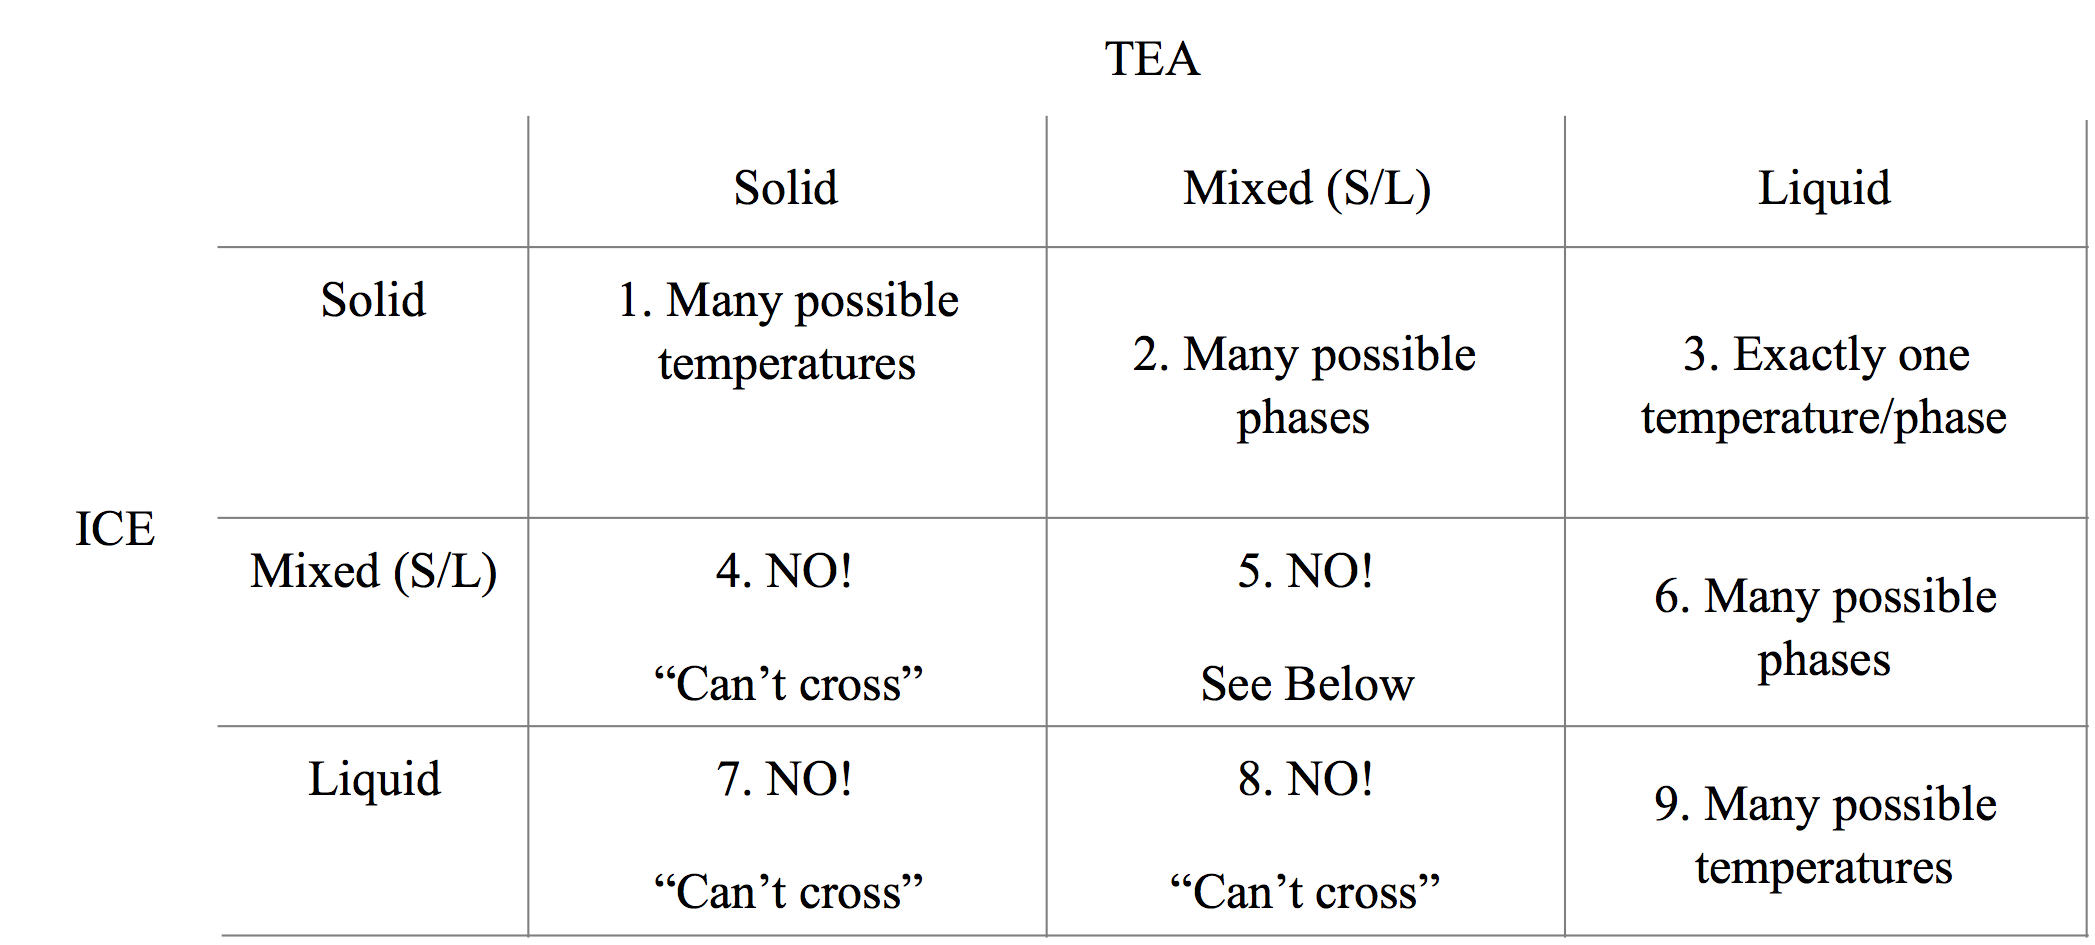
\includegraphics[width=.6\textwidth]{act123.png}
%	\end{center}
}

\WCD

	\item Now that we have a class consensus on which states are possible, your instructor will assign you one of the possible final states:
	\begin{enumerate}
		\item For your possible final state, draw an \EnergyDiagram{} (with energy conservation equation, as always).
		\item Would your final state be possible if there were A LOT of ice?  What about with A LOT of tea?

\WCD

	\end{enumerate}

	\bitem{Thinking about how to proceed:  How do we determine the final state?}
\note{}{
\textbf{Tell students the mass of the ice is 0.5 kg and the tea is 3.0 kg}
}	
	Put a \TempGraph{} on the board for each of the two systems: The water that starts out as ice at \unit[-65]{\textdegree C} and the tea (liquid water) that starts out at \unit[20]{\textdegree C}. Put a big dot on each graph at the initial state.
	
	\begin{enumerate}
		\item Have two separate group members place a finger on the two starting dots. Then a third group member should start explaining how energy is transferred from one physical system to the other, specifically naming the energy systems that are losing energy and that are gaining energy. Move the fingers along each graph in response to the explanation. Make sure every group member agrees with the explanation and the motion along the graphs. STOP when one substance gets to a phase change temperature.
		
		\item We need to use quantitative skills to figure out \textbf{which substance gets to its phase change temperature first}. With your group members, think about ways that you might be able to determine this. Hint: Are there two values you can compare? Write in words what you need to do to figure this out.
		\label{act123-compare-energies}
		
		\item After you have explained in words how you will figure out which substance gets to its phase change first, draw an \EnergyDiagram for each calculation you want to perform, and then perform the calculation.

\WCD 

		\note{}{
		No, it is not possible to determine the final state of the substances because we don�t know how much of each substance we have. Yes it is possible to eliminate some states: state 4, 5, 7, and 8 for the reasons listed in the chart. 
}	
		\item Is it possible to determine the final state of the substances yet?  Is it possible to eliminate any of the possible final states? Which one(s)?

		\item We now need to repeat \hyperref[act123-compare-energies]{Part~\ref*{act123-compare-energies}} to figure out which happens first: the tea decreases to \unit[0]{\textdegree C},  or the ice goes through an entire phase change. Draw {\em NEW initial points} and determine which changes in energy you need to compare. Then draw the \EnergyDiagrams, and do the calculations.
		
		\item Are the two physical systems in thermal equilibrium at the end of this step?  How do you know this?
		
		\item Can you now determine the final state of the ice and tea system? Draw an appropriate \EnergyDiagram on the board for this. If you finish early, you may solve for the final temperature or state.

\WCD

	\end{enumerate}
\end{enumerate}